\begin{frame}
	\frametitle{Atividades realizadas}
	\framesubtitle{Durante as ``férias''}
	
	\begin{itemize}
		\item Passagem de \destaq{MatLab} para \destaq{C++};
		\item \textit{Pipeline} para testar várias imagens de uma vez;
		\item Teste com imagens de banco de dados com folhas \cite{imageclef2011}, comparando escolha dos pontos âncora de maneira aleatória, linear ou por curvatura.
	\end{itemize}
	
\end{frame}


\begin{frame}
	\frametitle{Atividades realizadas}
	\framesubtitle{Exemplos de resultados (figura 6, 65 pontos)}
	
	\begin{figure}[ht!]
		\centering
		\begin{subfigure}[t]{0.24\textwidth}
			\centering
			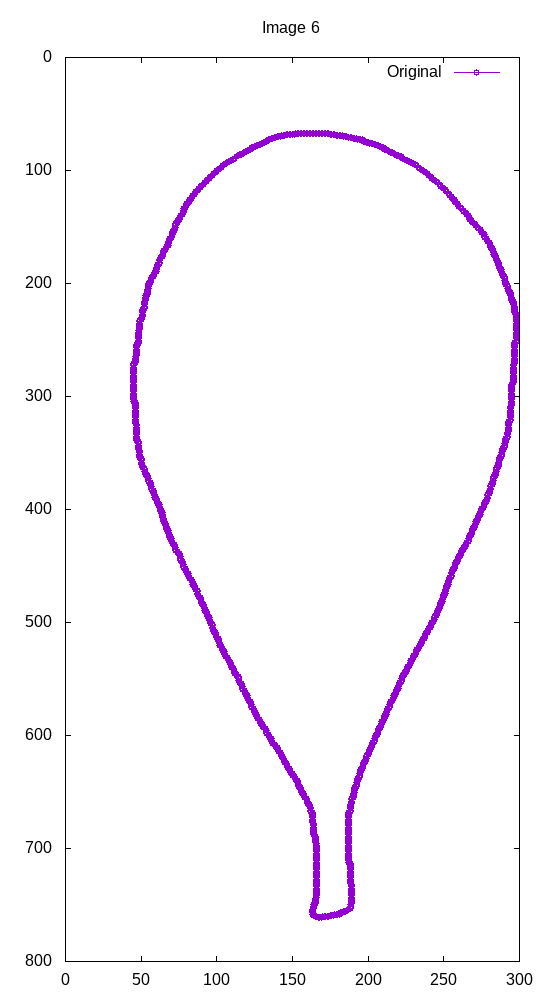
\includegraphics[width=\textwidth]{img/rec/6ori.png}
			\caption{Curva original}
		\end{subfigure}
		\begin{subfigure}[t]{0.24\textwidth}
			\centering
			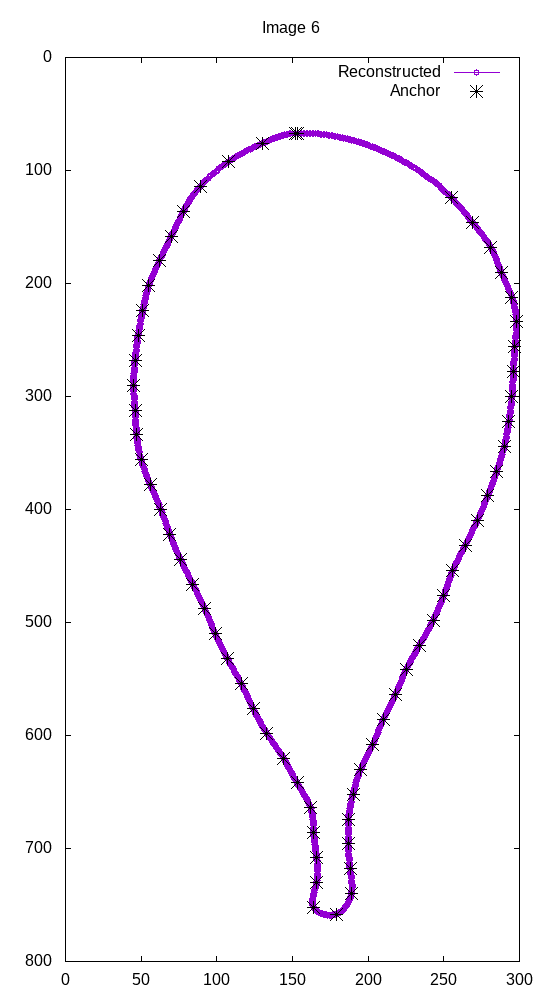
\includegraphics[width=\textwidth]{img/rec/6lin(781).png}
			\caption{Linearmente espaçados (781)}
		\end{subfigure}
		\begin{subfigure}[t]{0.24\textwidth}
			\centering
			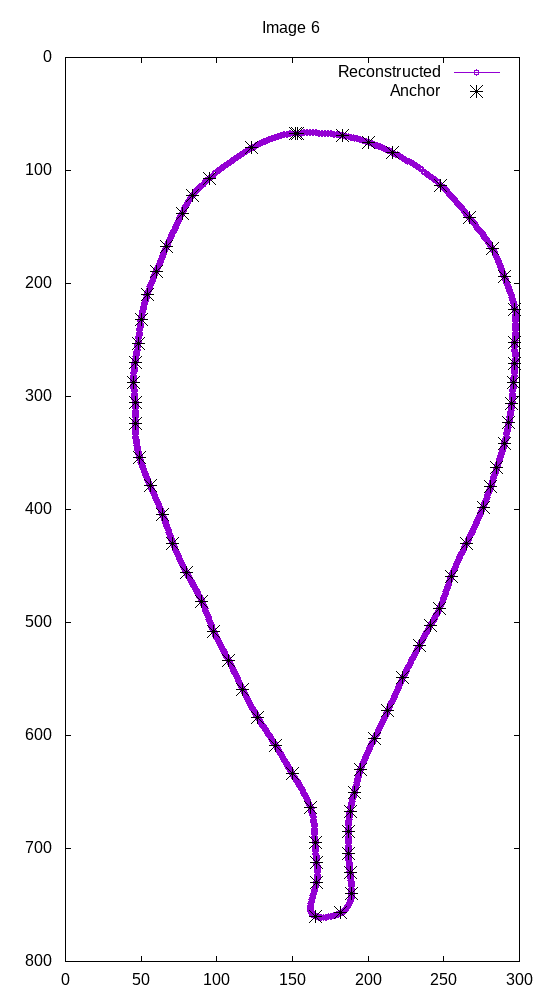
\includegraphics[width=\textwidth]{img/rec/6cur(663).png}
			\caption{Curvatura (663)}
		\end{subfigure}
		\begin{subfigure}[t]{0.24\textwidth}
			\centering
			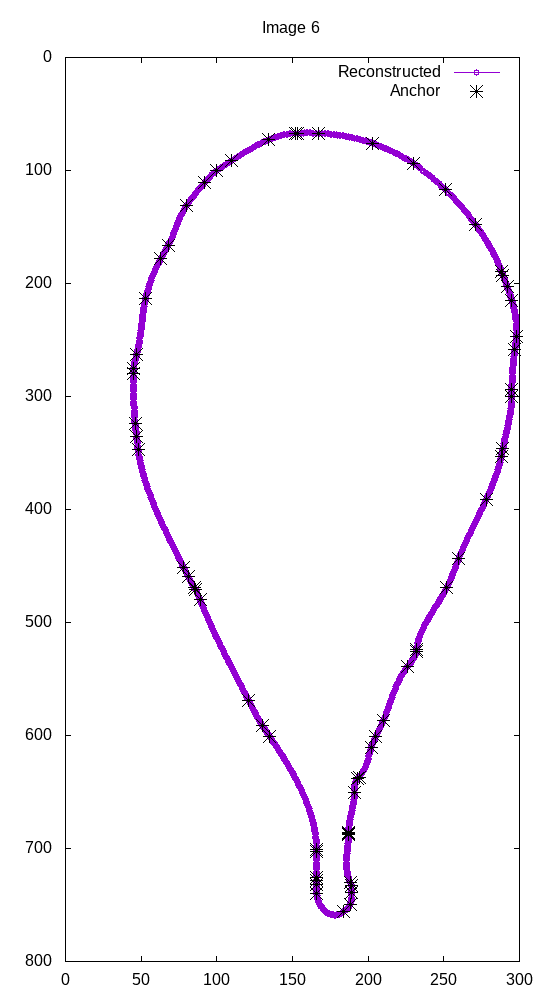
\includegraphics[width=\textwidth]{img/rec/6rng(1139).png}
			\caption{Aleatórios (1139)}
		\end{subfigure}
		\label{fig:rec6}
	\end{figure}
\end{frame}

\begin{frame}
	\frametitle{Atividades realizadas}
	\framesubtitle{Exemplos de resultados (figura 11, 65 pontos)}
	
	\begin{figure}[ht!]
		\centering
		\begin{subfigure}[t]{0.24\textwidth}
			\centering
			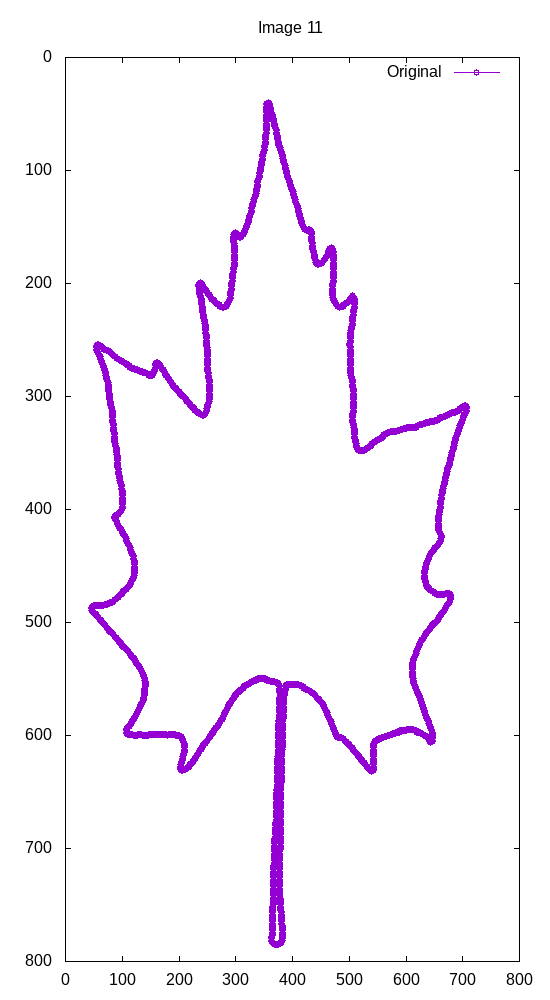
\includegraphics[width=\textwidth]{img/rec/11ori.png}
			\caption{Curva original}
		\end{subfigure}
		\begin{subfigure}[t]{0.24\textwidth}
			\centering
			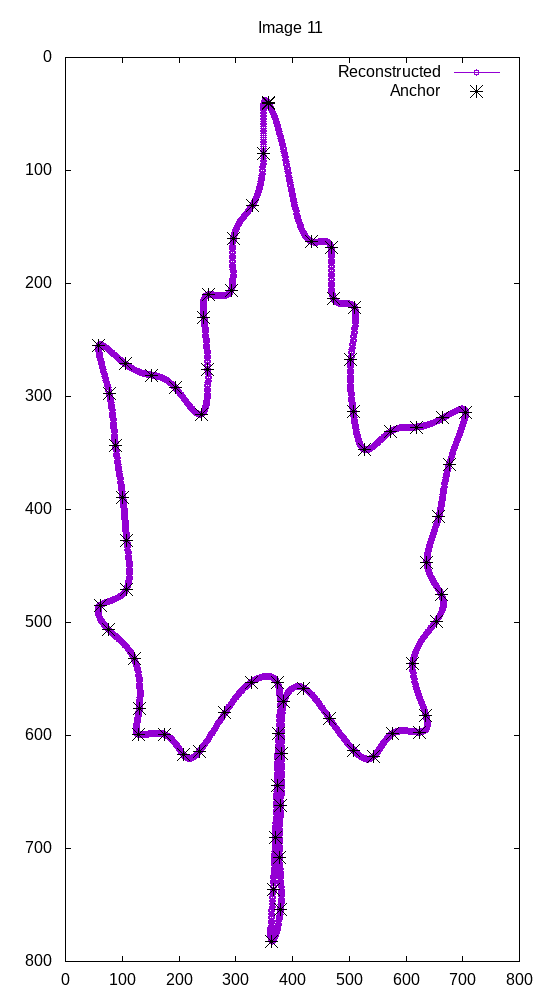
\includegraphics[width=\textwidth]{img/rec/11lin(11594).png}
			\caption{Linearmente espaçados (11594)}
		\end{subfigure}
		\begin{subfigure}[t]{0.24\textwidth}
			\centering
			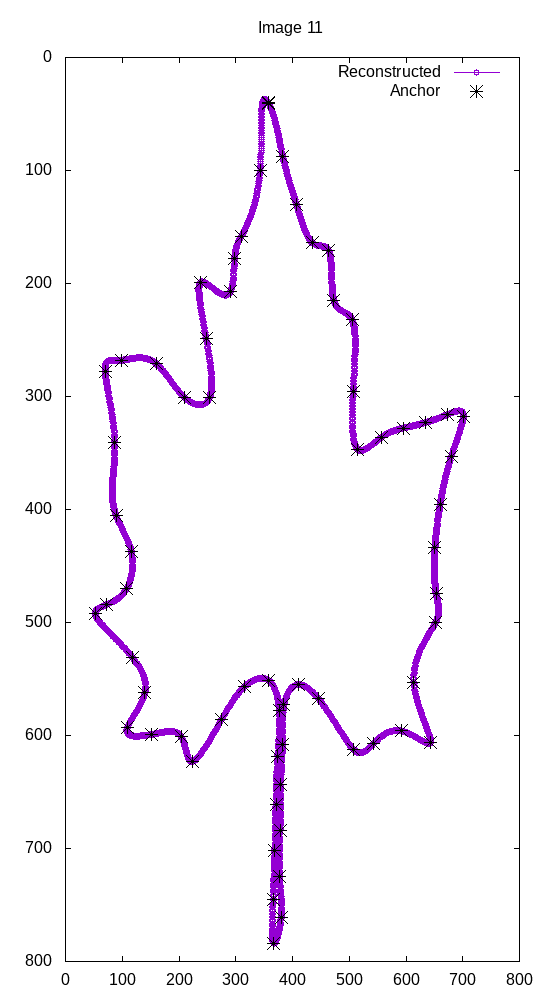
\includegraphics[width=\textwidth]{img/rec/11cur(13512).png}
			\caption{Curvatura (13512)}
		\end{subfigure}
		\begin{subfigure}[t]{0.24\textwidth}
			\centering
			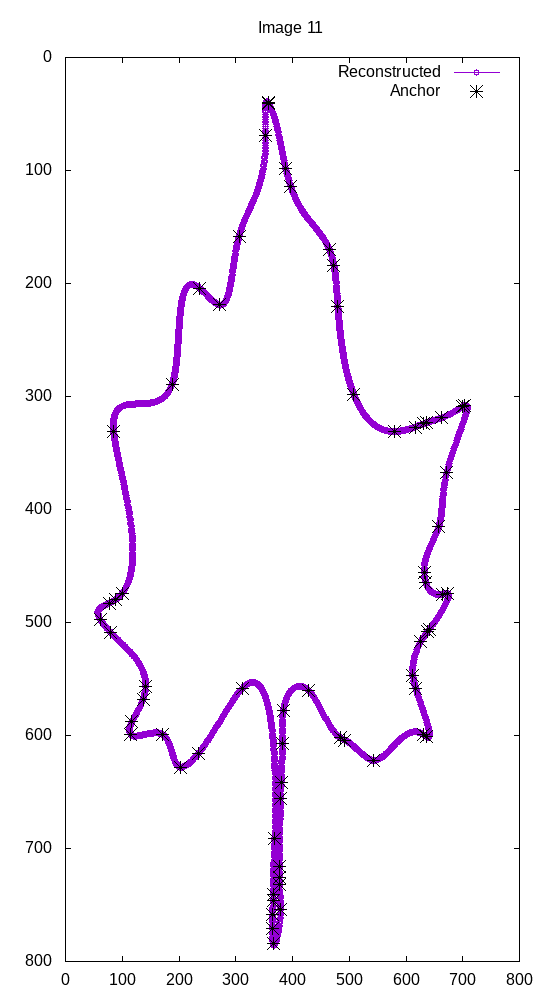
\includegraphics[width=\textwidth]{img/rec/11rng(32340).png}
			\caption{Aleatórios (32340)}
		\end{subfigure}
		\label{fig:rec6}
	\end{figure}
\end{frame}

\begin{frame}
	\frametitle{Atividades realizadas}
	\framesubtitle{Exemplos de resultados (figura 64, 65 pontos)}
	
	\begin{figure}[ht!]
		\centering
		\begin{subfigure}[t]{0.24\textwidth}
			\centering
			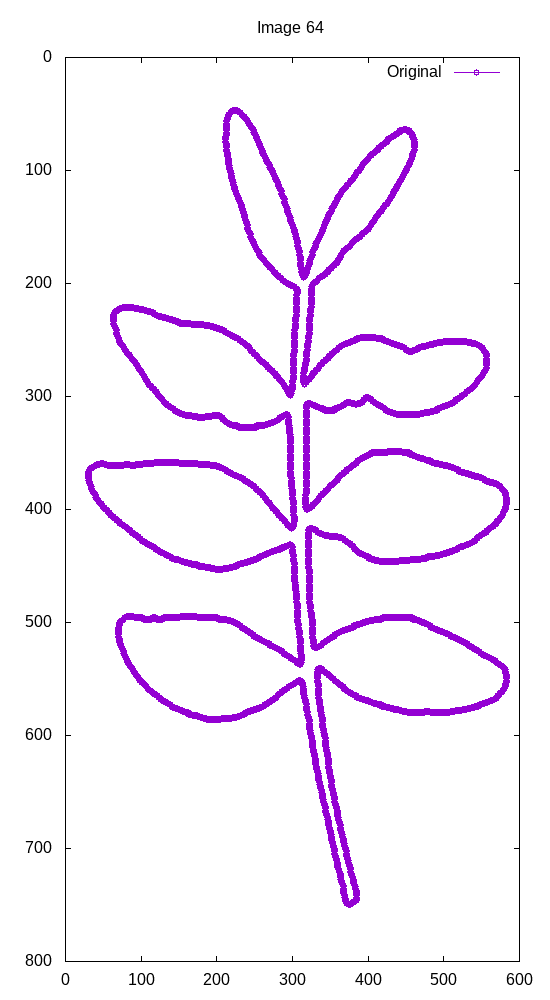
\includegraphics[width=\textwidth]{img/rec/64ori.png}
			\caption{Curva original}
		\end{subfigure}
		\begin{subfigure}[t]{0.24\textwidth}
			\centering
			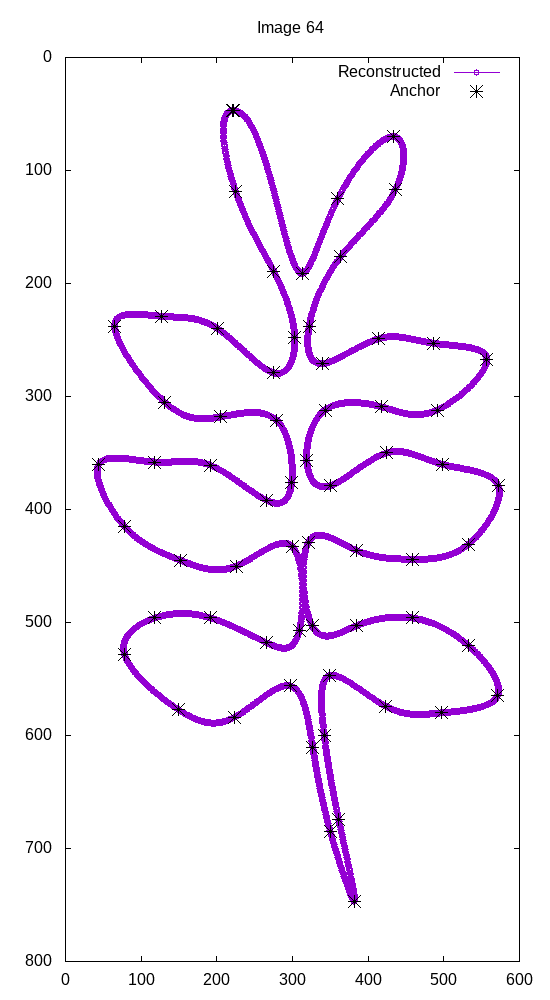
\includegraphics[width=\textwidth]{img/rec/64lin(24802).png}
			\caption{Linearmente espaçados (24802)}
		\end{subfigure}
		\begin{subfigure}[t]{0.24\textwidth}
			\centering
			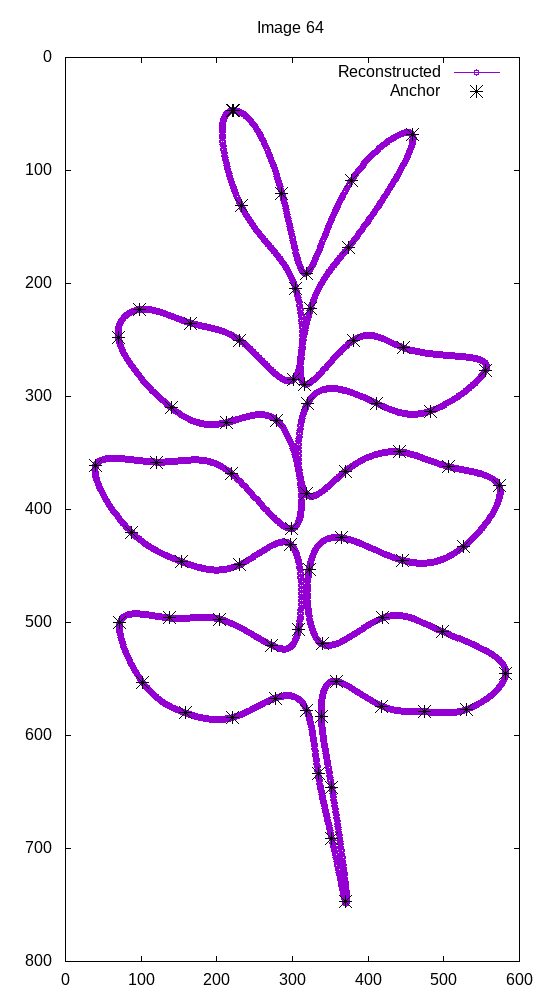
\includegraphics[width=\textwidth]{img/rec/64cur(26573).png}
			\caption{Curvatura (26573)}
		\end{subfigure}
		\begin{subfigure}[t]{0.24\textwidth}
			\centering
			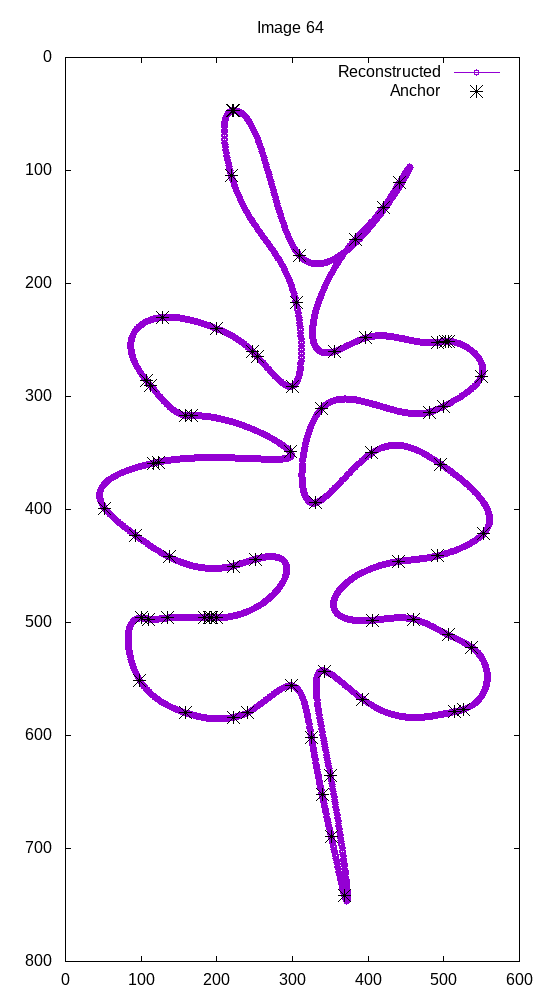
\includegraphics[width=\textwidth]{img/rec/64rng(50891).png}
			\caption{Aleatórios (50891)}
		\end{subfigure}
		\label{fig:rec6}
	\end{figure}
\end{frame}


